\documentclass[intern,palatino]{cgBA}

\author{Sebastian Gaida}
\title{Simulation von Rauch}
\zweitgutachter{Bastian Krayer MSc. }
\zweitgutachterInfo{(Institut für Computervisualistik, AG Computervisualistik)}
\externLogo{7.46cm}{logos/UniLogoNeu}
\externName{DIN: NewTechnologies}
\sloppy

\usepackage{acronym}
\usepackage{hyperref}
\usepackage{url}
\usepackage{listings}
\usepackage{xcolor}
\usepackage{float}
\usepackage{pgfplots}
\usepackage{subfigure}
\usepackage{caption}
\pgfplotsset{compat=1.16 ,legend style={at={(0.02,.98)},anchor=north west}}

\lstset{language=C++,
	frame=tb,
	tabsize=4,
	showstringspaces=false,
	numbers=left,
	commentstyle=\color{olive},
	keywordstyle=\color{blue},
	stringstyle=\color{red}
}

\setcounter{secnumdepth}{4}

\begin{document}

	\maketitle
	\newpage
	\pagenumbering{roman}
	
	
	%-------------------------------------------------------------------------------
	
	\section*{Abstract}\label{abstract}
	
	Diese Bachelorarbeit befasst sich mit der Simulation von Rauch mittels einem Partikelsystem. Hierbei werden die Möglichkeiten untersucht Rauch möglichst realistisch in einem Partikelsystem zu implementieren und in Echtzeit berechnen zu lassen. Die physikalische Simulation basiert dabei auf den Arbeiten von  Müller \cite{muller2003particle} und Ren \cite{ren2016fast}, welche sich mit den physikalischen Eigenschaften von Fluiden und Gasen beschäftigen. Die Simulation wurde mittels C++, OpenGL und der in OpenGL verfügbaren Compute-Shader auf der GPU implementiert. Dabei wurde ein besonderes Augenmerk darauf gelegt, dass diese möglichst performant ist. Hierfür werden Techniken von Hoetzlein \cite{nvidia} benutzt um das Partikelsystem zu beschleunigen. Daraufhin wurden zwei Beschleunigungsverfahren implementiert und werden noch gegenübergestellt. Dabei werden die Laufzeit, sowie verbrauchter Speicherplatz der GPU betrachtet.
	\newline \newline
	This bachelor thesis deals with the simulation of smoke in a particle system. Here the possibilities are investigated to implement smoke as realistically as possible in a particle system and to calculate it in real time. The physical simulation is based on the work of Müller \cite{muller2003particle} and Ren \cite{ren2016fast}, who deal with the physical properties of fluids and gases. The simulation was implemented on the GPU using C++, OpenGL and the compute shaders available in OpenGL. Special attention was paid to the performance of the simulation. Hoetzlein \cite{nvidia} techniques are used to accelerate the particle system. Two acceleration methods were then implemented and compared. The runtime, but also the used memory space of the GPU is discussed.
	
	\newpage
	
	\tableofcontents
	\clearpage
	\pagenumbering{arabic}
	\bibliographystyle{alphadin}
	\captionsetup{font=it}

%-------------------------------------------------------------------------------

\section{Vorwort}\label{vorwort}

Zur Simulation eines Fluids hat mich die Lehrveranstaltung Animation und Simulation inspiriert, da dort vermehrt Partikelsysteme implementiert wurden. Doch besaßen alle Simulationen eine schlechte Performance, weshalb nur wenige Partikel berechnet werden konnten. Mein persönliches Ziel war es deshalb, das System weites gehend zu beschleunigen.
\newline \newline
Vor dem Beginn der vorliegenden Bachelorarbeit möchte ich mich zunächst bei einigen Personen bedanken, die mich während der Arbeit unterstützt haben.
\newline \newline
Zunächst einmal bedanke ich mich bei Prof. Dr.-Ing. Stefan Müller und Bastian Krayer MSc. für die großartige Betreuung meiner Arbeit.
\newline
Danke  an alle, die sich die Zeit genommen haben meine Arbeit Korrektur zu lesen.
\newline
Außerdem möchte ich mich bei Pascal Bendler bedanken, der mich tatkräftig beim Debugging und Aufbau des Frameworks unterstützt hat.
\newline
Ein großes Dankeschön geht auch an Katharina Krämer, die mich immer wieder dazu motiviert hat weiter zu arbeiten und nach alternativen Möglichkeiten zu suchen.
\newpage

%-------------------------------------------------------------------------------

\section{Einleitung}\label{einleitung}

Das Ziel dieser Arbeit ist es eine möglichst physikalisch korrekte Rauchsimulation in einem Partikelsystem zu implementieren. Dazu wird die Tatsache genutzt, dass sich Rauch wie ein Fluid verhält \cite{stam2003real}, dabei wird die Simulation der physikalischen Basis von Fluiden angenähert. Es wird in dieser Implementation ein Partikelsystem zur Berechnung der physikalischen Eigenschaften genutzt. Echtzeit-Entwicklungsplattformen wie die Unity-Engine bieten zwar eine Partikelsimulation an, jedoch beschränkt sich diese lediglich auf das Ausstoßen von Partikeln. Dabei können Partikelinteraktionen, sowie Fluideigenschaften nicht angepasst werden.
\newline
Die GPU eignet sich besonders gut zum berechnen parallelisierbarer Rechenoperationen, da sie im Vergleich zur CPU, die nur wenige Kerne besitzt, über tausend Kerne verfügt. Diese sind zwar nicht so leistungsfähig wie die der CPU, bieten aber dennoch einen signifikante Steigerung der Leistung.
\newline
In der Arbeit wird auch darauf eingegangen den genannten Aufwand zu minimieren. Dazu wurden zwei Verfahren zur Beschleunigung des Partikelsystems auf der GPU implementiert und gegenübergestellt.
\newline
Für die Implementation wurde OpenGL genutzt, welches das programmieren auf der GPU deutlich vereinfacht und seit der Version 4.3 auch das verarbeiten von Daten mit Hilfe von Compute-Shadern unterstützt. Für den schnellstmöglichen Zugriff auf diese Daten wird Speicherplatz, in Form von SSBO, auf der GPU angelegt. Dabei sollte auch auf eine effiziente Nutzung des limitierten Speicherplatzes geachtet werden.

%-------------------------------------------------------------------------------

\section{State of the Art}\label{state}
Die Simulation zur Darstellung von Fluiden, ist ein jahrelange Herausforderung für die Computergrafik. Dabei treten immer wieder die gleichen Problemstellungen auf. Zum einen soll die Simulation physikalisch korrekt sein, um ein für den Beobachter möglichst schönes, sowie nachvollziehbares Ergebnis zu bieten. Schon kleinste Fehlverhalten, die von der Realität abweichen, können die Immersion zerstören. Andererseits soll das System auch in Echtzeit berechnet werden und dabei auf mögliche Interaktionen reagieren können. Für eine möglichst effiziente Berechnung werden verschiedene Beschleunigungsverfahren verwendet, die ein gutes Ressourcenmanagement in Form der Laufzeit, sowie Speicherplatz erfordern.
\newline \newline
Die physikalische Grundlage, die Navier-Stokes-Gleichungen, basiert dabei auf den Gleichungen die von Claude Louis Marie Henri Navier und George Gabriel Stokes im 19. Jahrhundert aufgestellt wurden. Diese Gleichungen beschreiben die physikalischen Eigenschaften von Fluiden und werden für die Simulation dieser angewendet. Diese Formeln werden je nach Fluid angepasst um speziellere Eigenschaften darzustellen\cite{temam1978navier}.
\newline
Diese Simulation wird meist in Form eines rasterbasierenden Verfahren oder eines Partikelsystems implementiert.
%-------------------------------------------------------------------------------

\subsection{Vektorfeldverfahren}\label{vektor}
Beim Vektorfeldverfahren wird die \textit{Umgebung} in gleichgroße Voxels unterteilt, auch bekannt als \textit{Voxelgrid oder eulersches Grid}. Bei diesem Vektorfeldverfahren betrachtet man die Partikel nicht direkt, sondern eine Masse, die in Form des Voxels generalisiert wird. Dabei werden Parameter, wie Dichte, Druck und Geschwindigkeit in dem jeweiligen Voxel gespeichert. Die Berechnungen lassen sich in Advektion, Druck, Diffusion und Beschleunigung unterteilen. Die Advektion beschreibt dabei den Strömungstransport, das Übertragen der Bewegungskraft auf ein anliegendes Objekt. Druck wiederum beschreibt die Übertragung von Kräften an benachbarte Partikel, wodurch bei einem zu hohen Druck eine Kraft vom Zentrum weg und wiederum bei einem Unterdruck eine Kraft zum Zentrum hin entsteht. Die Diffusion beschreibt die Viskosität des Fluides. Je nach Anpassung dieser breitet sich das Fluid stark, wie zum Beispiel Wasser, oder weniger stark wie Honig aus.
Bei Beschleunigung handelt es sich um eine externe Kraft die auf das Fluid wirkt, dies ist vergleichbar mit der Schwerkraft oder einer Windgeschwindigkeit. Zur Beschleunigung zählt man bei den Vektorfeldern aber auch die Wirbelkraft, die bei Rauch die typischen Turbulenzen verursacht und damit einen signifikanten Einfluss auf die Erscheinung hat.
\newline
Wegen der physikalisch präziseren Ergebnisse, eignet sich diese Verfahren besonders für Strömungsimulationen in Innenräumen \cite{franz}, da man Kraft einem System zuführt. Das Fluid, welchem die Kraft zugeführt wurde, wird daraufhin eingefärbt.
\newline
Bei dieser Methode stellt das Lösen der Gleichungen, zur Berechnung des Fluids, und die Visualisierung der Ergebnisse die größte Schwierigkeit dar. Die Visualisierung erweist sich als Hindernis, da in jedem Voxel Kräfte vorhanden sind. Dabei unterscheidet man in dem Grid unter einem gefärbten Teil und einem nicht sichtbaren Teil, der meist Luft repräsentiert, siehe Abbildung \ref{img:Vertexfeld}. Zur Darstellung des Fluides wird meist Volumerendering genutzt. Außerdem ist der Rechenaufwand hoch und lässt sich wegen der Grid-Architektur des Verfahrens nur schwer verbessern.

\begin{figure}[H]
	\centering
	\includegraphics[width=0.7\columnwidth]{Bilder/vektorfeld.jpg}
	\caption[Fluidsimulation in Form des Vektorfeldverfahren \newline Quelle:\url{https://thumbs.gfycat.com/CelebratedElasticHartebeest-poster.jpg}]{Fluidsimulation in Form des Vektorfeldverfahren}
	\label{img:Vertexfeld}
\end{figure}

%-------------------------------------------------------------------------------

\subsection{Partikelsystem}\label{partikel}

Bei dem Verfahren einer Partikelsimulation werden die Partikel einzeln betrachtet, dies bezeichnet man auch \textit{lagrangiansches Verfahren}. Diese speichern Parameter, wie Position und Geschwindigkeit selber ab. Die Berechnungen beschränken sich dabei auf die Dichte, Druck, Viskosität, Auftrieb und Wirbelkraft.
Die Nachbarpartikel werden dabei in die Berechnung miteinbezogen. Die Dichte beschreibt dabei, wie viele Nachbarpartikel Einfluss auf den betrachteten Partikel haben und wird als Gewichtung für die Berechnung der Kräfte verwendet. Das typische Verhalten des Fluides wird aber durch das Zusammenspiel der Kräfte Drucke und Viskosität erzeugt. Dabei sorgt der Druck dafür, dass die Partikel sich voneinander wegbewegen. Die Viskosität wirkt dem entgegen und führt das Anziehen von Partikel hervor. Der Auftrieb wiederum lässt sich über die Temperatur des Rauches bestimmen, welche je nach Dichte steigt oder sinkt. Zum anderen lässt sich aber die Wirbelkraft nicht so einfach berechnen und stellt somit ein Problem in der Forschung dar.
Für die Berechnungen werden die Nachbarpartikel benötigt, welche aber nicht für jeden Partikel bekannt sind. Es entsteht ein großer Aufwand, wenn man einfachheitshalber alle Partikel mit einbezieht. Hierbei entstehen viele Möglichkeiten das System zu optimieren.
\newline
Der Ansatz eines Partikelsystems eignet sich hervorragend zum Einbinden in eine Echtzeitanwendung. Wie beispielsweise ein Computerspiel oder Engine, da man mit der Partikelanzahl  die Performance beeinflussen kann. Beim Reduzieren der Partikel sollte eine Anpassung der Parameter erfolgen, da dies sonst einen signifikanten Einfluss auf das Verhalten des Fluides hat.
\newline
Die größten Schwierigkeiten bei einer Rauchsimulation in einem Partikelsystem entstehen durch die Beschleunigung der Nachbarschaftssuche, sowie den Auftrieb und die Wirbelkraft.
\begin{figure}[h]
	\centering
	\includegraphics[width=0.7\columnwidth]{Bilder/partikelsystem.jpg}
	\caption[Partikelsimulation von Wasser \newline \url{https://i.ytimg.com/vi/DhNt_A3k4B4/maxresdefault.jpg}]{Partikelsimulation von Wasser}
	\label{img:Partikelsystem}
\end{figure}

%-------------------------------------------------------------------------------

\section{Rauchsimulation}\label{rauch}

% Längeren Text
Zur Simulation von Rauch wurde ein Partikelsystem implementiert, dessen physikalische Grundlage auf dem Smooth-Particle-Hydordynamics-Verfahren(SPH) basiert. Dieses Verfahren verwendet Müller \cite{muller2003particle} 2003 zur Simulation von Fluiden. Dabei handelt es sich um eine Abwandelung der Navier-Stokes-Gleichungen für die Berechnung der Dichte, des Druckes und der Viskosität. Diese wurden zur Verwendung in einem SPH angepasst. Der Auftrieb, sowie die Temperaturberechung, stammen aus einem Paper von Ren \cite{ren2016fast}. Die größten Probleme bei der Implementation bereitete aber die Wirbelkraft. Ren und Macklin \cite{macklin2014unified} bieten eine Formel zur Berechnung dar, welche aber nicht das gewünschte Ergebnis lieferte.
\newline
Die Berechnung der Simulation bedarf Schritte die von einander abhängig sind. In Abbildung \ref{code:sim} werden alle Rechenschritte in einer optimalen Reihenfolge dargestellt. Die Berechnungen lassen sich in vier Compute-Shader unterteilen, welche voneinander abhängig und deshalb nicht weiter reduzierbar sind.
\newline
Zum Verständnis stellt die Abbildung \ref{tab:Symbole} alle Variablen dar, sowie deren Bedeutung und Format.

\begin{figure} [H]
	\centering
	\begin{lstlisting}
computeshader 1	
	for all particle i do
		for all neighbor of i do
			calculate density
		end for
		calculate pressure
	end for
end computeshader 1
computeshader 2
	for all particle i do
		for all neighbor of i do
			calculare normal
		end for
		calculate vorticity
	end for
end computeshader 2
computeshader 3
	for all particle i do
		for all neighbor of i do
			calculate pressure force
			calculate viscosity force
			calculate vorticity force
			calculate temperature
		end for
		calculate temperature cooldown
		calculate buoyancy force
		update velocity
	end for
end computeshader 3
computeshader 4
	for all particle i do
		apply velocity on position
	end for
end computeshader 4
	\end{lstlisting}
	\caption{Updateschleife der Physik}
	\label{code:sim}
\end{figure}

\begin{figure}[H]
	\centering
		\begin{tabular}{ | c | p{8cm} | c |}
			\hline
			Symbol & Bedeutung & Format  \\ \hline
			$m_i $ 				&  Masse des Partikel i								&	float	\\ \hline
			$r_i $		 		&  Position des Partikel i							&	vec3	\\ \hline
			$r_{ij}$ 			&  Abstandsvektor von $r_i - r_j$					&	vec3	\\ \hline
			$v_i$	 			&  Geschwindigkeitsvektor des Partikel i			&	vec3	\\ \hline
			$h $ 				&  Radius											&	float	\\ \hline
			$W_{ij} $ 			&  Gewichtungsfunktion, kurz für $W (r_i - r_j)$	&	float	\\ \hline
			$\nabla W_{ij} $ 	&  Gradienten-Gewichtungsfunktion					&	vec3	\\ \hline
			$\nabla^2 W_{ij} $ 	&  Laplace-Gewichtungsfunktion						&	float	\\ \hline
			$\rho_i $ 			&  Dichte des Partikel i		 					&	float	\\ \hline
			$\rho_0 $ 			&  Ruhedichte im Allgemeinen						&	float	\\ \hline
			$k $ 				&  Steifheit des Fluides							&	float	\\ \hline
			$p_i $ 				&  Druck des Partikel i								&	float	\\ \hline
			$f^{pressure}_i $	&  Druckkraft des Partikel i						&	vec3	\\ \hline
			$\mu $ 				&  Viskosität des Fluides							&	float	\\ \hline
			$\nu_i $ 			&  Viskosität des Partikel i						&	float	\\ \hline
			$f^{viscosity}_i $ 	&  Viskositätskraft des Partikel i					&	vec3	\\ \hline
			$T_i $ 				&  Temperatur des Partikel i						&	float	\\ \hline
			$D_r $ 				&  Zeit zum halbieren der Temperatur				&	float	\\ \hline
			$b $ 				&  Up-Vektor										&	vec3	\\ \hline
			$D_c $ 				&  Wärmeleitfähigkeitsfunktion des Fluides			&	float	\\ \hline
			$c $ 				&  Wärmeleitfähigkeit								&	float	\\ \hline
			$C_b $ 				&  Auftriebs-Koeffizient							&	float	\\ \hline
			$a_{b,i} $ 	  		&  Auftriebsbeschleunigung							&	vec3	\\ \hline
			$n_i $ 				&  Normale des Partikel i							&	vec3	\\ \hline
			$C_N $ 				&  nutzerdefinierter Schwellenwert					&	float	\\ \hline
			$y $ 				&  Zahl die nahezu 0 ist					 		&	float	\\ \hline
			$f^{buoyancy}_i $ 	&  Auftriebskraft des Partikel i					&	vec3	\\ \hline
			$\beta $ 			&  nutzerdefinierter Wert							&	float	\\ \hline
			$\omega_i $ 		&  Wirbelstärke des Partikel i						&	vec3	\\ \hline
			$f^{vortex}_i $ 	&  Wirbelkraft des Partikel i						&	vec3	\\ \hline
			$g $ 				&  Gravitationskraft								&	vec3	\\ \hline
			$ext $ 				&  externe Kraft									&	vec3	\\ \hline
			$\delta t $ 		&  Zeit seit letzter Iteration 						&	float	\\ \hline
			$\delta $ 			&  veränderte Wert im Abstand von $\delta t$ 		&			\\
			\hline
		\end{tabular}
	\caption{Bedeutung aller Symbole aller der Berechnungen}
	\label{tab:Symbole}
\end{figure}

%-------------------------------------------------------------------------------

\subsection{Gewichtungsfunktionen}\label{kernel}

Ein wichtige Aspekt, welchen Einfluss Nachbarpartikel auf den betrachteten Partikel hat, sind die Gewichtungsfunktionen. Diese bestimmen den Einfluss über die Entfernung $r_{ij}$ der Partikel zu einander, dabei spielt der Radius als Maximalabstand eine wichtige Rolle. Diese Funktionen besitzen alle die Eigenschaft, dass sie symmetrisch sind und beim Erreichen des Radius gegen 0 konvergieren. Damit haben zu weit entfernte Partikel keinen Einfluss mehr. Gewichtungsfunktionen dienen dazu eine Stabilität in das Partikelsystem zu bringen. Dabei nähern sie sich üblich Ableitungen von bestimmten Funktionen an \cite{muller2003particle}. Diese Funktionen wurden mit Hilfe von Bastian Krayer implementiert.
\newline
Für das SPH werden die drei folgenden Gewichtungsfunktionen genutzt. Abhängig von den Berechnungen wird eine andere Funktion für die richtige Stabilität des Systems benötigt. In Abbildung \ref{img:kernel} ist der Verlauf der Funktionen dargestellt.
\newline
Die $W_{poly}$-Funktion(\ref{funk:normal}) bietet einen weichen abfallenden Verlauf bei ansteigendem Abstand, diese Funktion wird als Standard für jegliche Berechnung genutzt.
\newline
Es werden aber für die Berechnungen ebenfalls ein Gradient, sowie ein Laplace benötigt. Der Gradient für die Druckberechnung lässt sich durch die Ableitung der für diese Berechnung vorgesehene Funktion berechnen. Mit der $W_{poly}$-Funktion wird beim Wert 1 ein nahezu 0 Wert erreicht. Dabei sollte dort die Druckkraft am höchsten sein.  Dies würde dazu führen, dass sehr nahe Partikel sich nicht mehr voneinander abstoßen würden. Deshalb nutzt Müller Desbrun \cite{desbrun1996smoothed} die Funktion(\ref{funk:gradient}), da diese in der Ableitung als Funktion(\ref{funk:gradient2}) Werte liefert, die für die Berechnung entsprechend konvergieren.
\newline\newline

\begin{equation}\label{funk:normal}
	W_{poly6}(r_{i,j}) = \frac{315}{64 \pi h^9}   
	\begin{cases}
	(h^2 - r^2)^3 		& 0	\leq r \leq h	\\
	0					& otherwise			\\
	\end{cases}
\end{equation}

\begin{equation}\label{funk:gradient}
W_{spiky}(r_{i,j}) = \frac{15}{\pi h^6}   
\begin{cases}
(h - r)^3 		& 0	\leq r \leq h	\\
0					& otherwise			\\
\end{cases}
\end{equation}

\begin{equation}\label{funk:gradient2}
\nabla W_{spiky}(r_{i,j}) = \frac{-45}{\pi h^6}   
\begin{cases}
(h - r)^2 		& 0	\leq r \leq h	\\
0					& otherwise			\\
\end{cases}
\end{equation}

\begin{equation}\label{funk:laplace}
W_{visc}(r_{i,j}) = \frac{15}{2 \pi h^3}   
\begin{cases}
-\frac{r^3}{2h^3} + \frac{r^2}{h^2} + \frac{h}{2r} -1  		& 0	\leq r \leq h	\\
0					& otherwise			\\
\end{cases}
\end{equation}

\begin{equation}\label{funk:laplace2}
\nabla ^2 W_{visc}(r_{i,j}) = \frac{45}{\pi h^6}
\begin{cases}
(h-r) 		& 0	\leq r \leq h	\\
0					& otherwise			\\
\end{cases}
\end{equation}

\begin{figure}[h]
	\centering
	\includegraphics[width=0.7\columnwidth]{Bilder/kernel.jpg}
	\caption{Die Gewichtungsfunktionen $W_{poly6}$, $W_{spiky}$, $W_{visc}$ nach \cite{muller2003particle} mit einem Radius von 1}
	\label{img:kernel}
\end{figure}
Die $W_{spiky}$-Funktion(\ref{funk:gradient}), würde aber wiederum in der zweiten Ableitung zu 0 werden. Bei anderen standardmäßigen Gewichtungsfunktionen könnte es sogar dazu führen, dass ein negativer Wert auftritt, der bei der Viskosität einen gegensätzlichen Effekt hätte. Deshalb wurde die $W_{visc}$-Funktion(\ref{funk:laplace}) entworfen, dessen Laplace(\ref{funk:laplace2}) optimal für die Berechnung der Viskosität ist.
\newline

\begin{figure}[H]
	\centering
	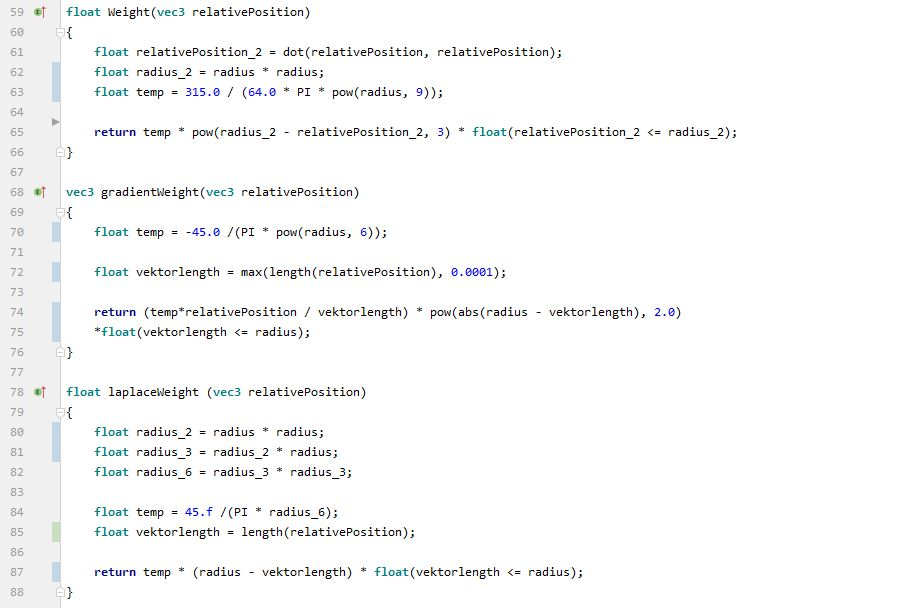
\includegraphics[width=1.35\columnwidth]{Bilder/impKernel.jpg}
	\caption{Implementation der SPH Kernel}
	\label{img:impkernel}
\end{figure}

In Abbildung \ref{img:impkernel} sind die Implementationen dargestellt. Dabei handelt es sich um die Funktionen $W_{poly6}$ in Zeile 59, $\nabla W_{spiky}$ in Zeile 68 und $\nabla^2 W_{visc}$ in Zeile 78.\newline
Die Abbruchfunktionen, wie in Formel(\ref{funk:normal}), (\ref{funk:gradient2}) und (\ref{funk:laplace2}) zu sehen, wird dabei durch die Multiplikation mit einer boolesche Variable durchgeführt, welche bei einem Abstand höher als dem Radius dazuführt, somit wird das Ergebnis 0.

%-------------------------------------------------------------------------------

\subsection{Dichte}\label{dichte}

Die Dichte ist eine Variable, die für jeden Partikel individuell berechnet wird. Sie beschreibt die Anzahl der Partikel in unmittelbarer Nähe zum betrachteten Partikel. Außerdem wird sie bei fast jeder folgenden Berechnung benötigt, da sie als Gewichtung des eingenommenen Volumens dient. 

\begin{equation}\label{funk:skalar}
A_s(r_i) = \sum_j m_j \frac{A_j}{\rho_j} W(r_i-r_j)
\end{equation}
\begin{equation}\label{funk:density}
\rho_i(r_i) = \sum_j m_j \frac{\rho_j}{\rho_j} W(r_i-r_j) = \sum_j m_j  W(r_{i,j})
\end{equation}

Die Dichte, wie in Gleichung(\ref{funk:density}) zu sehen ist, errechnet sich aus der Summe aller Nachbarn j. Dabei multiplizieren wird die Masse $m_j$ mit der Dichte $\rho_j$ durch die Dichte $\rho_j$ selbst. Dies wird dann noch mit der Gewichtungsfunktion, des Abstandes der Partikel, verrechnet. Die Gleichung ergibt sich aus der Berechnung für Skalaregrößen(\ref{funk:skalar}) von Müller \cite{muller2003particle}.
\newline\newline
Wie in Abbildung \ref{img:dichte} Zeile 90 erkennbar, ist die Masse der Partikel nicht vom jeweiligen Partikel abhängig. In dem Paper von Ihmsen \cite{ihmsen2014sph} wird eine Formel $m_i = h^3 \rho_0$ für die Masse vorgestellt, diese wird initial aufgerufen und die Masse ist für den Rest der Simulation gleichbleibend. Diese Formel hat sich aber als instabil in der Implementation herausgestellt. Deshalb wurde sie als Uniform-Variable implementiert, die bei allen Partikeln gleich ist. Der Vorteil dieser Implementation ist, dass man die Masse zu Beginn oder auch zur Laufzeit verändern kann. Wobei von einer Änderung während der Laufzeit abzuraten ist, da es zu einem instabilen Verhalten der Simulation führen kann.
\newline

\begin{figure}[H]
	\centering
	\includegraphics[width=1.35\columnwidth]{Bilder/dichte.jpg}
	\caption{Implementation der Dichtefunktion}
	\label{img:dichte}
\end{figure}

%-------------------------------------------------------------------------------

\subsection{Druck}\label{druch}

Die Druckkraft $f^{pressure}$ beschreibt das Abstoßen von Partikeln von einander. Die standardmäßige Berechnung für Skalaregrößen in Gleichung(\ref{funk:skalar}) ist aber in diesem Fall nicht symmetrisch und würde zu einer instabilen Simulation führen. Da für Partikel i nur der Druck $p$ des Nachbarpartikel j relevant wäre. Dies würde zu einer unterschiedlichen Druckkraft bei der Berechnung des Druckes zwischen den zwei Partikeln führen. Um dieses Problem zu umgehen, stellt Müller \cite{muller2003particle} eine alternative Formel(\ref{funk:pressureF}) vor, die eine symmetrische Berechnung zwischen den Partikeln ermöglicht. Dabei werden beide Druckwerte beider Partikel addiert, um das Verhältnis aber beizubehalten wird auch die Dichte im Nenner verdoppelt. Zur Gewichtung wird dabei die Gradientenfunktion(\ref{funk:gradient2}) genutzt. Damit der Vektor in die entgegengesetzte Richtung zum Partikel j zeigt, wird dieser negiert.
\newline
Zum Berechnen der Druckkraft muss aber zunächst der Druck berechnet werden. Die Formel(\ref{funk:pressure}) von Desbrun \cite{desbrun1996smoothed} wurde diesbezüglich angepasst, indem eine Ruhedichte von der eigentlichen Dichte abgezogen wurde. Dabei wird die Ruhedichte $p_0$ als Offset verwendet und hat keinen mathematischen Einfluss auf die Druckkraft \cite{muller2003particle}, da es diese nur um das Offset verschiebt. Die Variable $k$ beschreibt dabei die Steifheit und bestimmt wie stark sich der Rauch ausdehnt.

\begin{equation}\label{funk:pressure}
p_i = k(\rho - \rho_0)
\end{equation}
\begin{equation}\label{funk:pressureF}
f^{pressure}_i = - \nabla p(r_i) = - \sum_j m_j \frac{p_i+p_j}{2\rho_j} \nabla W(r_{i,j})
\end{equation}

%-------------------------------------------------------------------------------

\subsection{Viskosität}\label{visc}

Ein wichtiger Aspekt der Physik ist auch die Viskosität. Diese beschreibt den Einfluss der Kraft der umliegenden Partikel. Dabei haben aber nicht alle Partikeln gleich viel Einfluss auf einander. Daraus resultiert, dass die Viskosität eine asymmetrische Kraft ist. Wäre sie jedoch eine symmetrische Kraft würde es dazu führen, dass sobald sich eine große Anzahl an Partikel gleichzeitig in die selbe Richtung bewegen, sich diese ins unendliche beschleunigen würden. Dabei würde es bereits reichen, dass ein einzelner Partikel seine Kraft überträgt. Da dieser wie bei einem Dominoeffekt, alle Partikel in seiner Umgebung in seine Bewegungsrichtung beschleunigen. Um dies zu umgehen, modifiziert Müller \cite{muller2003particle} die SPH-Formel(\ref{funk:skalar}), indem der Unterschied des Geschwindigkeitsvektor $v$ in Betracht gezogen wird. Dies hat zur Folge, dass ein Partikel mit einem großen Geschwindigkeitsvektor trotzdem noch alle Partikel in seiner Nähe mit sich zieht, aber sich nicht mehr ins unendliche beschleunigen kann.
\newline
Dies lässt die Rauchsimulation wirken als würde er sich zusammenziehen. Daraus resultiert, dass die Partikel mit der angepassten Formel, sich auch abbremsen können, indem ein schnellerer Partikel beim Berechnen mit einem langsamen Partikel eine Viskositätskraft entgegen seiner Bewegungsrichtung erhält. 
\newline
Wie in der Formel(\ref{funk:visc}) wird der Geschwindigkeitsvektor des eigenen Partikel abgezogen. Als Gewichtungsfunktion wird dabei der Laplace(\ref{funk:laplace2}) der $W_{visc}$(\ref{funk:laplace}) genutzt.

\begin{equation}\label{funk:visc}
f^{visc}_i  = \mu \sum_j m_j \frac{v_j-v_i}{\rho_j} \nabla^2 W(r_{i,j})
\end{equation}

Die Variable $\mu$ beschreibt die eigentliche Viskosität. $\mu$ ist bei Fluiden wie Honig hoch und bei Rauch sehr gering. In der Implementation hat $\mu$ deshalb einen sehr geringen Wert von $0.25$.

%-------------------------------------------------------------------------------

\subsection{Auftrieb}\label{auftrieb}

Auftrieb ist eine Kraft, die abhängig von der Temperatur des Rauches ist. Oftmals wird diese Temperatur statisch implementiert und eine Berechnung dieser vermieden. Dabei ist zu beachten ist, dass die Partikel sich bei einer hohen Dichte gegenseitig aufheizen und bei einer niedrigen abkühlen. Um dieses Verhalten umzusetzen wurde die Auftriebsvariante von Ren \cite{ren2016fast} implementiert.
\newline
Zum Anpassen der Temperatur der Partikel wurde die Formel(\ref{funk:temp}) verwendet. Diese betrachtet die Nachbarpartikel und heizt bzw. kühlt die Partikel, abhängig der Nachbarn, auf oder ab. Bei dieser Formel fehlte aber eine Definition der Funktion Dc, weshalb diese durch Formel(\ref{funk:thermal}) ersetzt wurde. Diese multipliziert den Temperaturunterschied mit einer Konstanten $C$ die den Wärmestrom des Rauches beschreibt. $\gamma$ ist dabei nur eine Variable, die positiv und nahe 0 ist, die das Teilen durch 0 verhindert.
\newline
Die Formel(\ref{funk:temp2}) beschreibt zudem das Abkühlen von Partikeln, die kaum bis keine Nachbarpartikel haben. Dafür wird die Temperatur durch die Zeit geteilt, die benötigt wäre um die Temperatur zu halbieren. Welche Partikel dabei betroffen sind wird über die Normale $n_i$ ermittelt, dazu wird die Formel(\ref{funk:normale}) verwendet. Die Normale wird bei einer geringen Dichte $\rho$ größer und wenn diese einen nutzerdefinierten Schwellwert, überschreitet führt dies zur Abkühlung des Partikel. Leider lässt sich diese Formel nur bei einer positiven Temperatur anwenden, welches das Abkühlen von bereits negativer Temperatur verhindert.
\newline
Wenn die Temperatur errechnet wurde lässt diese sich wie in Formel(\ref{funk:temp3}) berechnen. Dabei beschreibt $b$ einen Up-Vektor und $C_b$ den Auftriebs-Koeffizienten.

\begin{equation}\label{funk:thermal}
Dc(T)  = C * T
\end{equation}

\begin{equation}\label{funk:temp}
\frac{\delta T_i}{\delta t}  = \sum_j \frac{m_j}{\rho_i \rho_j} Dc(T_i - T_j) \frac{(r_i-r_j) \cdot \nabla W_{i,j}}{(r_i-r_j)^2 + \gamma^2}
\end{equation}

\begin{equation}\label{funk:normale}
n_i  = \sum_j \frac{m_j}{\rho_j} \nabla W_{i,j}
\end{equation}

\begin{equation}\label{funk:temp2}
\frac{\delta T_i}{\delta t}  = - T_i/D_r
\end{equation}

\begin{equation}\label{funk:temp3}
f^{buoyancy}_i  = C_b T_i b
\end{equation}

%-------------------------------------------------------------------------------

\subsection{Wirbelkraft}\label{wirbel}

Die Wirbelkraft ist die schwierigste zu berechnende Kraft in einem SPH. In dem Paper von Ren \cite{ren2016fast} wird eine Art beschrieben und ebenfalls die von Macklin \cite{macklin2014unified} erwähnt.
\newline
Ein Bestandteil der Wirbelkraft ist die Wirbelstärke, die sich aus dieser und dem Geschwindigkeitsgradienten, sowie der Normalen und der Gravitation errechnen lässt, Formel(\ref{funk:wirb}). Bei dem Geschwindigkeitsgradienten ist aber zu beachten, dass dieser eine Jacobi-Matrix der Geschwindigkeit ist und dort eine Matrixmultiplikation mit der Wirbelstärke stattfindet. Um den Gradienten anzunähern, wird wie von Macklin \cite{macklin2014unified} empfohlen ein SPH-Gewichtungsfunktion(\ref{funk:gradient2}) zu nutzen. Diese Formel beschreibt den Abstand des Partikel zu der Oberfläche des Rauches, dabei repräsentiert ein hoher Wert die Oberflächenpartikel und ein kleiner die inneren Partikel.
In der Formel(\ref{funk:wirb2}) wird dann noch die Wirbelstärke der umliegenden Partikel mit dem Abstandsvektor als Vektorprodukt verrechnet, um einen Vektor zu erhalten der eine Verwirbelung innerhalb des Fluides verursachen soll.  
\begin{equation}\label{funk:wirb}
\frac{\delta \omega_i}{\delta t}  = \omega_i \cdot + \nabla v + \beta(n_i \times g)
\end{equation}

\begin{equation}\label{funk:wirb2}
f^{vortex}_j  = \sum_j (\omega_j \times (r_i -r_j)) W_{i,j}
\end{equation}

Eine Wirbelkraft zu errechnen, welche die Turbulenzen verursacht ist leider nicht gelungen. Diese hatte lediglich die Wirkung, dass der Rauch langsamer aufgetrieben ist. Das langsame Ausstoßen von Partikeln hat leider keine positiven Auswirkungen auf die Physik. Dadurch entstanden eher Instabilitäten des Drucks, welcher sich zu Beginn anpassen lies, aber dann inkonstant wurde. Eine Anpassung der Variablen führte leider dabei zu keinem Erfolg. Es wurden auch andere Versuche unternommen die Wirbelkraft anzupassen, wie unter anderem die Formel zu modifizieren, welche aber erfolglos blieben.

%-------------------------------------------------------------------------------

\subsection{Update Kräfte}\label{kräfte}

Abschließend werden alle Kräfte zusammengerechnet und zum Geschwindigkeitsvektor hinzugefügt, Formel(\ref{funk:update}). Ein Spezialfall dabei ist die Gravitation, die mit der Dichte verrechnet wird. Zusätzlich können auch externe Kräfte $ext$ hinzugefügt werden um bestimmte Umwelteinflüsse zu simulieren. Dabei beschränkt es sich lediglich auf einen Vektor der bei allen Partikeln gleichstark wirkt.
\newline

\begin{equation}\label{funk:update}
\frac{\delta v_i}{\delta t}  = f^{pressure}_i + f^{viscosity}_i + f^{buoyancy}_i + f^{vortex}_i + ext + \rho_i g
\end{equation}

%-------------------------------------------------------------------------------

\section{Implementierung}\label{imp}

Bei der Implementierung wurde darauf geachtet, dass das System einfach und schnell anpassbar ist, um das Testen zu vereinfachen.
Dazu können einige Parameter während der Laufzeit angepasst werden. Hierfür wurde ImGui \cite{ocornut} verwendet, welches eine UI, siehe Abbildung \ref{img:ext}, zur Verfügung stellt, um die Parameter anzupassen.
Das Anpassen der Variablen während der Laufzeit kann aber zur Instabilität der Physik führen.
\newline
ImGui diente auch dazu die Laufzeit der einzelnen Berechnungsschritte dazustellen. Aus diesen Informationen konnten unter anderem darauf geschlossen werden, welche Berechnungen besonders viel Aufwand mit sich bringen. Diese Zeiten machten aber auch darauf aufmerksam, das ein Prozess, der einen geringen Aufwand haben sollte, trotzdem eine hohe Laufzeit benötigte. Daraufhin wurden im Countingsort \ref{counting} beim Umorganisierungschritt eine Anpassung vorgenommen, die sich positiv auf die Leistung ausgewirkt hat.

\begin{figure}[H]
	\centering
	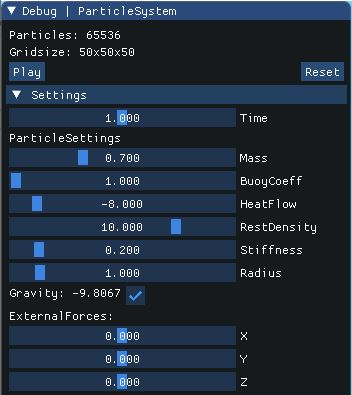
\includegraphics[width=0.35\columnwidth]{Bilder/external.jpg}
	\caption{Anpassbare Variablen per ImGui}
	\label{img:ext}
\end{figure}

Damit bei dem Iterieren über das eigene Grid ein Partikel sich nicht selbst beeinflussen kann wurde, wie in Abbildung \ref{img:normal} Zeile 88-90 zu sehen ist, ein Bedingung eingebaut. Diese verhindert es, dass ein Partikel mit derselben ID einen Einfluss auf sich selbst, nehmen kann. Auf die Begrenzung der Nachbarn, die in die Berechnung eingenommen werden, wird in Abschnitt \ref{vergleich} eingegangen.
\newline
Da die Implementierung die GPU verwendet muss darauf geachtet werden, dass die angewendeten Verfahren auch parallel berechenbar sind. Da nicht alle Kerne der GPU gleich schnell arbeiten, muss verhindert werden, dass Werte die von anderen Prozessen noch gelesen wird, nicht überschrieben werden.
Um dieses Problem zu umgehen wurden zwei identische Shader Storage Buffer Objects (SSBOs) für die Partikel angelegt, welches zwar mehr Speicheraufwand bedeutet, aber bei ca. 65.000 Partikel nur zusätzlich 12 MB beträgt. Bei den zwei SSBOs werden diese im Wechsel zum lesen un schreiben genutzt \ref{img:flipflop}. Dadurch besitzt das lesbare SSBO die zuletzt berechneten Daten und schreibt die neuen in das beschreibbare SSBO, hierbei wird aber immer anfangs das beschreibbare zunächst mit dem lesbaren SSBO überschrieben, damit alle Daten aktuell sind.
Es muss dabei aber auch auf eine gerade Anzahl der Aufrufe der Compute-Shader geachtet werden, da sonst im Beginn der Update-Schleife aus dem falschen SSBO gelesen wird. Hierfür wurde ein simpler Compute-Shader implementiert, der nur das alte SSBO mit den Daten des neuen überschreibt.
\newline
Für das parallele Schreiben in das gleiche SSBO bedarf es aber wiederum speziellen Operationen, die verhindern, dass mehrere Zugriffe gleichzeitig passieren und eine Variable bearbeiten. Dieses Problem entsteht häufig beim Versuch der Beschleunigung, da dort viele parallele Prozesse der Partikel auf das SSBO des Grids zugreifen.
\newline
OpenGL bietet in GLSL dabei Atomic-Operationen an, diese verhindern, dass ein anderer Prozess ebenfalls auf die Variable zugreift und diese bearbeitet. Dies entsteht dadurch, dass diese Funktionen zunächst einmal überprüfen, ob die Variable bereits bearbeitet wird, falls dies der Fall ist, wird solange gewartet bis sie freigegeben wird. Durch viele Prozesse, die auf eine Variable zugreifen wollen, können dadurch Warteschlangen für diese entstehen, woraus ein Zeitverlust resultiert.

\begin{figure}[H]
	\centering
	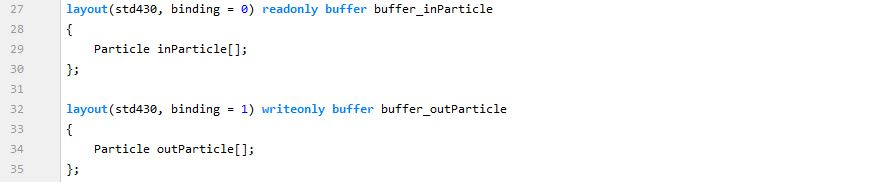
\includegraphics[width=1.3\columnwidth]{Bilder/Flipflop.jpg}
	\caption{Partikel SSBOs zum lesen und schreiben}
	\label{img:flipflop}
\end{figure}
%-------------------------------------------------------------------------------

\section{Beschleunigung}\label{besch}

Um ein Partikelsystem in einer Engine zu integrieren, muss diese möglichst performant sein, da in einer Engine auch andere Prozesse berechnet werden. Es bestehen mehrere Möglichkeiten ein Partikelsystem zu beschleunigen, eine liegt darin die zu betrachtenden Nachbarpartikel zu begrenzen. Durch die Gewichtungsfunktionen \ref{kernel} werden ohnehin Partikel die außerhalb des Radius $h$ liegen nicht mehr miteinbezogen. Würde man einfach über alle möglichen Nachbarpartikel iterieren, würde ein $O(n^2)$ Aufwand anfallen, hierbei steht n für die Anzahl der Partikel. Dies würde bei 1000 Partikeln ein Aufwand von 1.000.000 Rechenoperationen pro Rechnung pro Frame bedeuten. Dies ließe sich nicht in Echtzeit berechnen, geschweige denn in eine Engine integrieren. Deshalb wurden im folgenden Abschnitt die Möglichkeiten, diese Laufzeit zu reduzieren, untersucht und gegenübergestellt.  

%-------------------------------------------------------------------------------

\subsection{gridbasierte Nachbarschaftssuche}\label{nachbar}

Eine Möglichkeit die Laufzeit zu verringern basiert darauf, dass man nur die Nachbarn mit in die Berechnung einbezieht, die infrage kommen. Dafür müsste man aber alle Partikel miteinander vergleichen, die Nachbarn für einen einzigen Partikel herausfinden und für diese Iteration abspeichern. Dies ist mit einem noch hohem Aufwand, sowie einem großen Speicherverbrauch verbunden sein. Bei diesem wäre nicht klar, wie viel Speicher benötigt wird, da die Anzahl der Nachbarpartikel nicht bekannt ist. Man müsste dabei vom Worst-Case ausgehen und genug Speicherplatz für alle Partikel anlegen.
\newline
Hoetzlein \cite{nvidia} stellt dabei eine gridbasierte Nachbarschaftssuche vor. Diese lässt sich in die folgenden 3 Unterpunkte unterteilen.

\begin{enumerate}
	\item Unterteilen der Welt in gleichgroße Gridbehälter
	\item Hinzufügen der Partikel in die Gridbehälter
	\item Suche der Partikel in den Nachbarbehältern 
\end{enumerate}

Der 1. Punkt wird bereits beim Initialisieren durchgeführt, dabei wird vorher vom Benutzer vorgegeben wie groß die Griddimensionen sein sollen. Dieser Wert ist zu Laufzeit nicht mehr anpassbar, da die Gridbehälter(Grid) als SSBO angelegt wird. Jedes Grid besitzt eine eindeutige ID die gleich mit der $gl\_GlobalInvocationID.x$ in dem Compute-Shader ist. 
\newline
Punkt 2 bedarf einer hohen Menge an Speicherplatz, da davon ausgegangen werden muss, dass im Worst-Case-Szenario sich alle Partikel in einem Grid aufhalten. Welches bei einer Gridgröße von $50x50x50$ und ca. $65.000$ Partikel $32,5$ GB verbrauchen würde, dies wäre noch ineffizienter, da das anlegen des Speicherplatzes für alle potenziellen Nachbarn, bei allen Partikeln, weniger verbrauchen würde. Dabei handelt es sich bei diesen Zahlen um eine Simulation, die später als Standardsimulation betrachtet wird.
\newline
Ein Problem dabei ist aber auch, dass die Partikel zunächst zugeordnet werden müssen. Dies erfolgt über die in Abbildung \ref{img:lable} in Zeile 46 zu findende Funktion $cubeID$, welche über die Position des Partikel eine eindeutige GridID ausrechnet. Das Hinzufügen der Partikel, in die Grids ist je nach Verfahren unterschiedlich und wird genauer in Abschnitt \ref{counting} und \ref{speicher}  erklärt.
\newline
In Punkt 3 handelt es sich lediglich um ein iterieren über alle Partikel in den Nachbarbehältern, da diese bereits stark eingegrenzt wurden und durch die Gewichtungsfunktionen nur die Partikel betrachtet werden die in dem entsprechenden Radius sind.
\newline
In Abbildung \ref{img:grid} sieht man ein vereinfachtes 2D-Grid mit einem Partikel, welcher dem Grid in der Mitte zuzuordnen ist. Bei einem standardmäßigem Radius $h$ von 1, werden alle möglichen Nachbarpartikel, die infrage kommen abgedeckt. Hierbei werden alle 9 in 2D oder 27 in 3D Grids betrachtet und über die Partikel in diesen iteriert.

\begin{figure}[H]
	\centering
	\includegraphics[width=1\columnwidth]{Bilder/grid.jpg}
	\caption{Partikel im Grid mit einem Radius von 1}
	\label{img:grid}
\end{figure}

Diese Art der Nachbarschaftssuche besitzt einen Aufwand von $O(n k)$ im Optimalfall, wobei k die Anzahl der Nachbarpartikel ist. Da aber der Speicheraufwand extrem hoch ist, kommt diese Art der Nachbarschaftssuche leider nicht in Frage und es wird von Hoetzlein \cite{nvidia} eine alternative Suche mit einem Sortieralgorithmus vorgeschlagen.
\newline
Dabei werden die Partikel den Grids zugeordnet, diese wiederum Speichern die Anzahl der Partikel aller vorherigen Grids und wie viele Partikel sie selbst beinhalten. Damit wird dann über einen Sortieralgorithmus bestimmt, an welcher Stelle die Partikel zu welchem Grid im Speicher gehören. Dann muss nur noch von einem Grid die erste Speicheradresse, sowie die Anzahl der Partikel abgefragt werden und über diese iteriert werden.
\newline
In Abschnitt \ref{counting} wird genauer auf ein solches Verfahren, sowie die Implementation, eingegangen.

%-------------------------------------------------------------------------------

\subsection{Speicherverfahren}\label{speicher}

Beim Speicherverfahren wird ein großer Aufwand an Speicherplatz auf der GPU benötigt. Da dieser aber begrenzt und deshalb nicht für große Simulationen verwendbar ist, wird eine Begrenzung des genutzten Speicherplatzes angewendet. Heinrich \cite{nvidia2} beschreibt, dass bei der Implementation von Müllers \cite{muller2003particle} Fluidsimulation nur 32 Nachbarnpartikel für eine korrekte Simulation von Nöten sind, die einen Einfluss auf den betrachteten Partikel haben. Da ein ausgeglichener Einfluss auf diesem Partikel herrschen soll, wurden die Nachbarn nicht auf 32 Partikel beschränkt, sondern auf 16 Partikel pro Grid. Dadurch können maximal 432 Partikel in die Berechnungen mit einbezogen werden. Wobei, man in Abbildung \ref{img:grid} sehen kann, dass nicht alle Grids durch die Gewichtungsfunktionen \ref{kernel} mit einbezogen werden. Im Durchschnitt haben pro Nachbarschaftssuche ca. 138 Nachbarpartikel einen Einfluss auf die Berechnung.
\newline
Bei der Implementation wurde einfachheitshalber bei den Grids 16 unsigned int Variablen hinzugefügt, die die IDs der Nachbarpartikel beinhaltet.
\newline
Wie in Abbildung \ref{img:Storinglable} zu sehen, werden die zunächst die Zugehörigkeiten der Partikel zu dem Grid berechnet. Daraufhin wird mit der $count$ Variable berechnet, an welcher Speicherposition die IDs der Partikel gespeichert wird. Dafür wird wegen der parallelen Prozesse eine Atomic-Funktion genutzt, woraufhin Partikel, die einen Wert unter 16 besitzen, in dem Grid an der entsprechenden Position gespeichert werden. Es werden daraufhin bei der Nachbarschaftsbetrachtung nur noch die abgespeicherten IDs abgerufen. 

\begin{figure}[H]
	\centering
	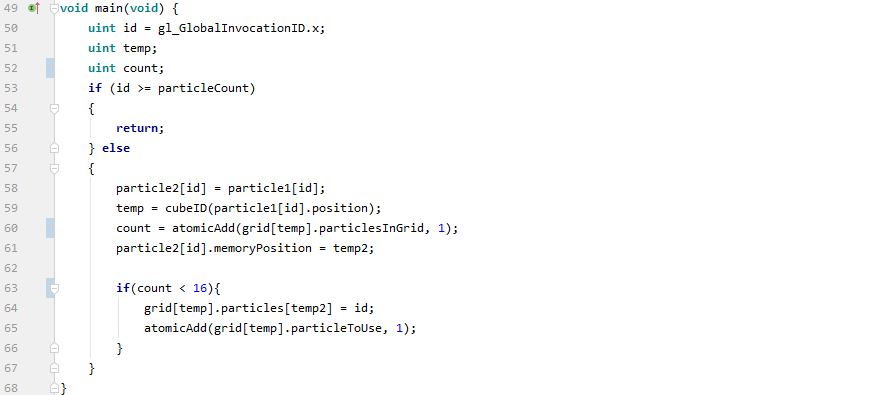
\includegraphics[width=1.3\columnwidth]{Bilder/StoringLable.jpg}
	\caption{Speichern der Partikel-IDs im Grid }
	\label{img:Storinglable}
\end{figure}

Diese Form der Nachbarschaftsbetrachtung besitzt in der Theorie einen Aufwand von $O(n k)$. Was aber dabei nicht beachtet wurde ist, dass die Partikel-IDs in den Grids sich sehr stark unterscheiden können, wie in Abbildung \ref{tab:Speicher} zu sehen.
\newline
Durch diesen unsortierten Speicher entstehen sogenannte \textit{scattered reads}, diese Art den Speicher auszulesen ist um einiges langsamer als bei einem sortierten Speicher. Dies entsteht durch, den Zugriff auf Speicheradressen die einen großen Abstand besitzen.
\newline
Dieses Verfahren ist allerdings noch um einiges schneller, als die Brute-Force-Methode.

\begin{figure}[H]
	\centering
	\begin{tabular}{ | c || c | c | c | c | c | c | c | c | c |}
		\hline
		Grid 				&  20 & 16 & 13 & 20 & 20 & 13 & 16 & 18 & 15	\\ \hline
		Speicherposition	&   0 &  1 &  2 &  3 &  4 &  5 &  6 &  7 &  8	\\
		\hline
	\end{tabular}
	\caption{Unsortierter Speicher beim Speicherverfahren}
	\label{tab:Speicher}
\end{figure}

%-------------------------------------------------------------------------------

\subsection{Sortierverfahren}\label{sortieren}
Um das Problem der \textit{scattered reads} zu beheben, müssen die Speicherpositionen nach dem Grid sortiert werden \ref{tab:Speichersorted}, damit ein Speicherzugriff erfolgen kann der möglichst kompakt ist. Dafür wird aber ein Sortieralgorithmus benötigt. Ein sequentieller Algorithmus würde aufgrund der Architektur der GPU sich dafür nicht eignen, da diese zwar viele Kerne besitzt, die gemeinsam eine große Rechenleistung, aber einzeln nur eine geringe besitzen. Dort wäre es effizienter die Daten wieder auf die CPU zu übertragen und dort sortieren zu lassen.

\begin{figure}[H]
	\centering
	\begin{tabular}{ | c || c | c | c | c | c | c | c | c | c |}
		\hline
		Grid 				&  13 & 13 & 15 & 16 & 16 & 18 & 20 & 20 & 20	\\ \hline
		Speicherposition	&   2 &  5 &  8 &  1 &  6 &  7 &  0 &  3 &  4	\\
		\hline
	\end{tabular}
	\caption{sortierter Speicher nach Sortieralgorithmus}
	\label{tab:Speichersorted}
\end{figure}

Da das Sortieren auf der CPU aber sequentiell ist, würde es wertvolle Laufzeit verbrauchen, ebenfalls das Übertragen der Daten auf die CPU. Deshalb wird ein paralleler Sortieralgorithmus auf der GPU benötigt, Hoetzlein \cite{nvidia} stellt dabei zwei Sortierverfahren gegenüber. Der erste ist RadixSort, dieser Sortieralgorithmus bezieht sich auf das Betrachten der einzelnen Stellen einer Zahl und sortiert anhand dessen. Dadurch, dass jeder Kern eine einzelne Zahl betrachten und diese dann einordnen kann, mach diesen Sortieralgorithmus parallelisierbar.
RadixSort hat einen Aufwand von $O(l n)$, wobei l für die Anzahl der Stellen steht. Laut diesem Aufwand ist er damit schneller als der zweite Algorithmus CountingSort mit einem Aufwand von $O(n log(n))$. Jedoch benötigt laut Hoetzlein \cite{nvidia} RadixSort 15 Kernel calls und CountingSort nur 4 Kernel calls pro Frame. Dadurch ist CountingSort trotz größerem Aufwand der schnellere Algorithmus, auf dessen Theorie und Implementation im folgenden Abschnitt näher eingegangen wird.

%-------------------------------------------------------------------------------

\subsection{Countigsort}\label{counting}
Countingsort ist ein nicht vergleichsbasierter Algorithmus, sondern ist adressenbasiert. Dabei dürfen nur natürliche Zahlen als Schlüsselwert in dem Array vorkommen, welche mit einem maximalen Wert begrenzt werden.
Dies erlaubt eine parallele Implementation, bei der die Laufzeit unabhängig von der Zuordnung des Arrays ist und damit eine festen Aufwand hat.
Die einzelnen Schritte des Sortieralgorithmus erfolgen nach Demaine \cite{counting}.
\newline
Für den Countigsort wird ein Array mit den zu sortierenden Zahlen wie in der Tabelle \ref{tab:Counting1} benötigt, dabei muss die maximale Größe des Wertes im Array bekannt sein.
\newline

\begin{figure}[H]
	\centering
	\begin{tabular}{ | c || c | c | c | c | c |}
		\hline
		Index 				&  0 & 1 & 2 & 3 & 4 \\ \hline
		Wert				&  8 & 2 & 5 & 3 & 5 \\
		\hline
	\end{tabular}
	\caption{Ausgangsarray beim Countingsort}
	\label{tab:Counting1}
\end{figure}

Zunächst werden dann in einem Hilfsarray die Anzahl der vorkommenden Werte bestimmt (Abb.\ref{tab:Counting2}). Daraufhin wird die Summe aus allen vorherigen Anzahlen bestimmt und in das Hilfsarray geschrieben (Abb.\ref{tab:Counting3}).
\newline

\begin{figure}[H]
	\centering
	\begin{tabular}{ | c || c | c | c | c | c | c | c | c | c | c |}
		\hline
		Wert 				& 0	&  1 & 2 & 3 & 4 & 5 & 6 & 7 & 8 & 9	\\ \hline
		Anzahl				& 0 &  0 & 1 & 1 & 0 & 2 & 0 & 0 & 1 & 0	\\
		\hline
	\end{tabular}
	\caption{Anzahl der Werte im Hilfsarray}
	\label{tab:Counting2}
\end{figure}

\begin{figure}[H]
	\centering
	\begin{tabular}{ | c || c | c | c | c | c | c | c | c | c | c |}
		\hline
		Wert 				& 0	&  1 & 2 & 3 & 4 & 5 & 6 & 7 & 8 & 9	\\ \hline
		Anzahl				& 0 &  0 & 1 & 2 & 2 & 4 & 4 & 4 & 5 & 5	\\
		\hline
	\end{tabular}
	\caption{Summe der Anzahl der Werte im Hilfsarray}
	\label{tab:Counting3}
\end{figure}

Zuletzt wird über die Werte des initialen Array iteriert und der Wert an die Anzahl der Summe minus 1 geschrieben, dies beruht darauf, dass die Arrays mit dem Index 0 starten und hat keinen Zusammenhang mit dem folgenden Schritt. Daraufhin wird die Summe der Anzahl bei diesem Wert um 1 verringert, aber bei den folgenden Zahlen nicht angepasst. Dadurch kann eine Zahl mehrfach vorkommen und wird trotzdem richtig einsortiert.
\newline

\begin{figure}[H]
	\centering
	\begin{tabular}{ | c || c | c | c | c | c |}
		\hline
		Index 				&  0 & 1 & 2 & 3 & 4 \\ \hline
		Wert				&  2 & 3 & 5 & 5 & 8 \\
		\hline
	\end{tabular}
	\caption{vollständig sortiertes Array}
	\label{tab:Counting4}
\end{figure}

%Implementierung
%-------------------------------------------------------------------------------

Bei der Implementation mussten Anpassungen zwischen dem vorgeschlagenen Algorithmus von Hoetzlein \cite{nvidia} und der Theorie von Demaine \cite{counting} vorgenommen werden. Diese erfolgten für eine schnellere und stabilere Implementation des Sortieralgorithmus, außerdem liefert Hoetzlein bloß einen groben Aufbau des Algorithmus, welcher als Grundlage des Aufbaus diente, siehe Abbildung \ref{code:Counting}.
\newline

\begin{figure}[H]
	\centering
	\begin{lstlisting}
computeshader 1
	for all grid i do
		reset grid
	end for
end computeshader 1
computeshader 2
	for all particles i do
		lable Particles to Grid
	end for
end computeshader 2
computeshader 3
	for all grid i do
		init gridBuffer
	end for
end computeshader 3
for log_2(ParticleCount) do
	computeshader 4
		for all grid i do
			calculate PrefixSum
		end for
	end computeshader 4
	computeshader 5
		for all grid i do
			update gridBuffer
		end for
	end computeshader 5
end for
computeshader 6
	for all particles i do
		rearrange Particles
	end for
end computeshader 6
	\end{lstlisting}
	\caption{Aufbau des Implementierten Countingsort}
	\label{code:Counting}
\end{figure}

Der Sortieralgorithmus beginnt mit dem Zurücksetzen des Grid-SSBOs (Abb.\ref{img:GridStruct}). Dies dient dazu, dass die  Berechnung des vorherigen Frames keinen Einfluss hat. Dabei werden alle Variablen bis auf die ID zurückgesetzt, wobei die ID und der $previousSortOutPut$ Füllervariablen sind um die 16 Byte zu erreichen, sie haben aber noch einen Mehrwert im Debugging.

\begin{figure}[H]
	\centering
	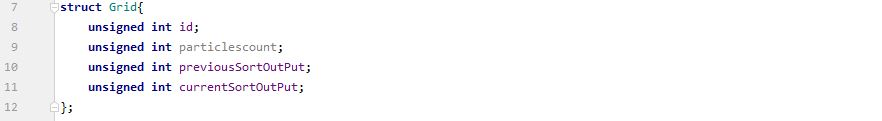
\includegraphics[width=1.3\columnwidth]{Bilder/GridStruct.jpg}
	\caption{SSBO-Struct des Grids}
	\label{img:GridStruct}
\end{figure}

Im Folgenden wird die Anzahl der Partikel in einem Grid gespeichtert, die Zugehörigkeit zum Grid wird über die CubeID-Funktion ermittelt, welches in Abbildung \ref{img:lable} in Zeile 60 zu sehen ist. Eine atomicAdd-Funktion wird dabei durchgeführt und es wird der Wert $grid[temp].particlesInGrid$ um 1 erhöht. In $outParticle[id].memoryPosition$ wird der Wert vor der Addition gespeichert und dieser sagt aus als wievielter sich dieser Partikel im Grid registriert hat. Die Abwandelung mit dieser Variable spart beim $rearrange Particles$-Schritt kostbare Laufzeit.

\begin{figure}[H]
	\centering
	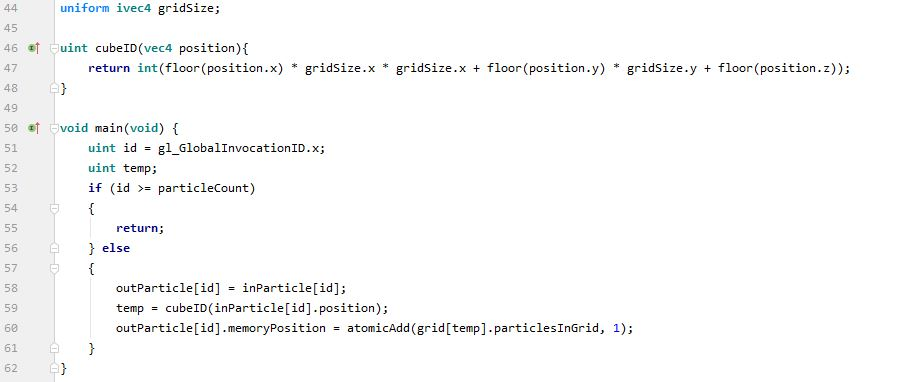
\includegraphics[width=1.3\columnwidth]{Bilder/lable.jpg}
	\caption{registrieren der Partikel im Grid mit CubeID-Funktion }
	\label{img:lable}
\end{figure}

Zum Berechnen der Prefixsum wird der parallele Scan von Nav\"{i}e nach Harris \cite{harris2007parallel} implementiert. Dieser berechnet die Prefixsum über die Summe der bisherigen Anzahl der $i - 2^d$ Nachbarn, wobei $d = 0$ to $log_2(n)-1$.

\begin{figure}[H]
	\centering
	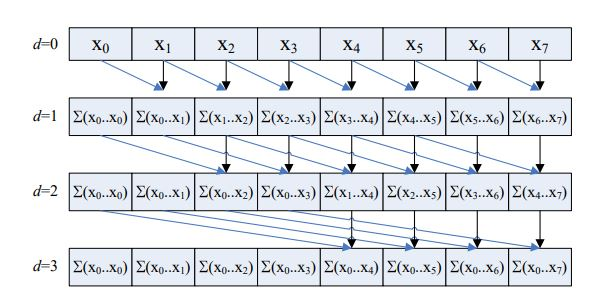
\includegraphics[width=1.0\columnwidth]{Bilder/PrefixSum.jpg}
	\caption{paralleler Prefixsum Scan von Nav\"{i}e nach Harris \cite{harris2007parallel}}
	\label{img:prefixsum}
\end{figure}

Um den ersten Schritt zu vereinfachen und keinen Zugriff auf Variablen zu haben, die überschrieben werden könnten, wird der Algorithmus damit initialisiert, dass die Anzahl der Partikel die sich im Grid befinden in den $currentSortOutPut$ sowie in den Gridbuffer geschrieben wird.
\newline
Der Gridbuffer dient in dem Fall als temporärer Buffer, der bloß eine Float-Variable speichert, damit nicht gleichzeitig aus einem Buffer die gleiche Variable gelesen und beschrieben wird.
Dafür werden die Compute-Shader zu Berechnung der Prefixsum und zum updaten des Gridbuffers im wechsel $log_2(Particleanzahl)-1$ durchgeführt. Bei der Prefixsum wird aus dem Gridbuffer die aktuelle Summe plus die Summe des $i - 2^d$ Nachbarn addiert und in dem $currentSortOutPut$ des Grid-SSBOs gespeichert. Daraufhin wird der Gridbuffer aktualisiert und es wird die Summe, die in der $currentSortOutPut$ Variable steht, übertragen.
\newline
Im letzten Schritt müssen die Partikel nur noch neu angeordnet werden. Dies müsste nach dem Algorithmus für jedes Grid sequentiell ablaufen, damit sich die Partikel nacheinander an die richtige Position schreiben. Dies entspricht dem Schritt von Abbildung \ref{tab:Counting3} zu \ref{tab:Counting4}.
\newline
Um diesen sequentiellen Prozess zum umgehen, wurde aber im Vornherein bereits in der $outParticle[id].memoryPosition$ die Position des Partikels im Grid bestimmt. Deshalb können die Partikel, wie in \ref{img:rearrange} zu sehen, sich bloß an die entsprechende Speicherstelle schreiben. Diese Anpassung spart ca. 0,1ms pro Frame bei 65.000 Partikeln. Dadurch befinden sich nun alle Partikel, die in einem Grid sind in aufeinanderfolgenden Speicherplätzen und verhindert damit \textit{scattered reads}.

\begin{figure}[H]
	\centering
	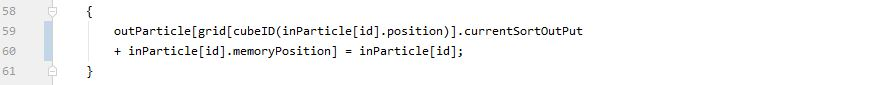
\includegraphics[width=1.3\columnwidth]{Bilder/rearrange.jpg}
	\caption{umorganisieren der Partikel im Speicher}
	\label{img:rearrange}
\end{figure}

Das Aufrufen der Nachbarpartikel erfolgt daraufhin, wie zum Beispiel, bei der Normalenberechnung (Abb.\ref{img:normal}). Dabei wird zunächst die $id$ des Nachbargrids über die $CubeID$-Funktion ermittelt. Daraufhin wird der $currentSortOutPut$ des Nachbargrids, welcher dem ersten Partikel in dem Grid entspricht, als initial Wert der For-Schleife genommen. Diese läuft bis die Summe des $currentSortOutPut$ plus die $particlesinGrid$ erreicht worden sind oder eine andere Abbruchbedingung eintritt.

\begin{figure}[H]
	\centering
	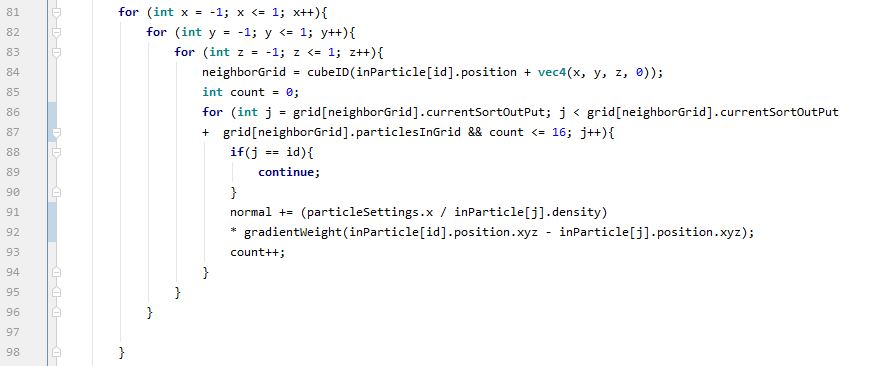
\includegraphics[width=1.3\columnwidth]{Bilder/normal.jpg}
	\caption{Berechnung der Normalen einen Partikel}
	\label{img:normal}
\end{figure}

%-------------------------------------------------------------------------------

\subsection{Vergleich}\label{vergleich}

Die beiden Beschleunigungsverfahren bieten auf Kosten von Speicherplatz und Laufzeit eine sehr starke Verkürzung der Laufzeit. Im Folgenden werden beide Beschleunigungsverfahren gegenübergestellt und mit einander auf Vor- und Nachteile untersucht.
\newline
Damit bei beiden Verfahren über gleich viele Partikel iteriert wird und dies damit keinen Einfluss auf die Beschleunigung hat, wurde der Countingsort ebenfalls auf 16 Partikel pro Grid beschränkt (Abb.\ref{img:normal}). Als Standardwerte für die Partikelanzahl wird $65.536$ und für die Gridgröße $50x50x50$ angesehen, welche bei speziellen Tests für die Partikel oder das Grid dann variieren können.
\newline
Die Tests wurden auf einem Desktop-Pc mit einer Intel(R) Core(TM) i5-9600k CPU @ 4.0 GHz und einer Nvidia GeForce GTX 1660 Ti Grafikkarte durchgeführt. Bei den Tests wurden die Durchschnittswerte von 20s Laufzeit pro Simulation ausgewertet. Bei den zeitlichen Angaben handelt es sich um Millisekunden pro Frame.
\newline
Beim Vergleich der Sortieralgorithmen bei steigender Partikelanzahl (Abb.\ref{tab:particle}) haben beide eine ähnliche Berechnungsdauer bei einer niedrigen Anzahl, dabei ist aber der Countingsort bereits ein wenig schneller. Besonders bemerkbar macht sich der Unterschied bei hoher Partikelanzahl bei dem das Speicherverfahren fast die doppelte Laufzeit pro Frame besitzt. Dies ist ganz klar auf die scattered reads zurückzuführen, die das Speicherverfahren, trotz weniger Kernal calls, erheblich verlangsamen. Beim Countingsort deutet es einen linearen Verlauf der Laufzeit an, wie es Hoetzlein \cite{nvidia} beschreibt. Diese Linearität scheint aber zwischen 525.000 und 1.000.000 nicht mehr gegeben zu sein. Dies liegt höchstwahrscheinlich an der Datenübertragungsrate der Grafikkarte. Da es bei einer mit höherer Datenübertragungsrate und vergleichbar vielen Kernen zwar ebenfalls keine perfekte Linearität aufwies, aber eine deutlich besseren Verlauf zeigte. Leider konnten keine eindeutigeren Tests auf dieser Grafikkarte durchgeführt werden, da diese nur kurz zur Verfügung stand.  

\begin{figure}[H]
	\centering
	\begin{tabular}{ | c || c | c | c | c | c | c | c | c |}
		\hline
		Partikel			&  8.912 & 16k & 32k & 65k & 131k & 262k & 524k & 1kk	\\ \hline
		Countingsort														\\ \hline
		Laufzeit(ms)		&   0,72 &  1,27 &  2,13 &  4,12 &  12,71 &  27,81 &  56,72 &  142,56		 	\\ \hline
		
		Speicher															\\ \hline
		Laufzeit(ms)		&   0,9 &  1,88 &  3,69 &  7,34 &  15,15 &  38,71 &  107.45 &  270,65	\\
		\hline
	\end{tabular}
	\caption{Laufzeit in Relation zur Partikelanzahl}
	\label{tab:particle}
\end{figure}

Einen Einfluss auf die Laufzeit hat auch die Griddimension, wobei dieser sehr viel geringer ausfällt als die der Partikelanzahl. Wie in Abbildung \ref{tab:Grid} zu sehen, ist auch hier der Countingsort schneller und bei diesem haben die Griddimensionen auch weniger Einfluss auf die Laufzeit, als beim Speicherverfahren. Bei dem Speicherverfahren steigt die Laufzeit stärker an, obwohl dieser Anstieg sich nicht signifikant von dem des Countingsort unterscheidet.

\begin{figure}[H]
	\centering
	\begin{tabular}{ | c || c | c | c | c | c | c | c | c | c |}
		\hline
		Partikel			&  20 & 30 & 40 & 50 & 60 & 70 & 80 & 90 & 100	\\ \hline
		Countingsort														\\ \hline
		Laufzeit(ms)		&   5,85 &  4,43 &  3,92 &  4,04 &  4,27 &  4,54 &  4,85 &  5,37 &	6,36	 	\\ \hline
		
		Speicher															\\ \hline
		Laufzeit(ms)		&   7,4 &  7,04 &  7,14 &  7,45 &  8,47 &  9,29 &  9.54 &  9,84 & 10,41	\\
		\hline
	\end{tabular}
	\caption{Laufzeit in Relation zur den Griddimensionen}
	\label{tab:Grid}
\end{figure}

Das Sinken und anschließende Steigen aus Abbildung \ref{tab:Grid} lässt sich durch das stärkere Verteilen der Partikel erklären, da sich in einem kleineren Raum mehr Partikel in einem Grid befinden und sich dadurch mehr atomicAdd-Funktionen bei den einzelnen Grids stauen.

\begin{figure}[H]
	\centering
	\begin{tikzpicture}
		\begin{axis}[width=1.0\textwidth,height=0.5\textheight]
		\addplot[smooth,mark=*,blue]
		coordinates {
			(20,30.158) (30,30.656) (40,31.376) (50,32.569) (60,34.345) (70,36.826) (80,40.126) (90,44.365) (100,49.658)
		};
		\addlegendentry{Countingsort}
		\addplot[smooth,color=red,mark=x]
		coordinates {
			(20,26.681) (30,28.237) (40,31.271) (50,36.276) (60,43.740) (70,54.158) (80,68.021) (90,85.823) (100,108.053)
		};
		\addlegendentry{Speicherverfahren}
		\end{axis}
	\end{tikzpicture}
	\caption{Speicherverbrauch in Kb auf der Y-Achse und Griddimensionen auf der X-Achse }
	\label{dia:speicher}
\end{figure}

Da der Speicherplatz der Grafikkarte nicht unbegrenzt ist, lohnt es sich ebenfalls einen Blick auf diesen zu werfen in Verbindung mit den Griddimensionen, da diese sich bei den Sortieralgorithmen im nutzenden Speicher unterscheiden (Abb.\ref{dia:speicher}).
\newline
Zunächst hat das Speicherverfahren einen geringeren Verbrauch, welcher daraus resultiert, dass für den Countingsort neben dem Grid-SSBO noch der temporäre Gridbuffer als SSBO existiert. Doch beim Speicherverfahren steigt der benötigte Speicherplatz sehr viel stärker an als beim Countigsort. Bei diesem ist nur ein geringer Anstieg zu verzeichnen.

%-------------------------------------------------------------------------------
\newpage

\section{Ergebnis}\label{ergebnis}

In der Studienarbeit wurde gezeigt, dass die Realisierung einer Rauchsimulation mit Hilfe eines Partikelsystem bedingt möglich ist. Hierbei weißt das simulierte Fluid einige Eigenschaften von Rauch auf. Der Auftrieb, so wie Druck und Viskosität verhalten sich physikalisch korrekt. Die Wirbelkräfte in einer Rauchsimulation zu realisieren, welche auf einem Partikelsystem basiert, benötigt jedoch eine komplexere Berechnung. Diese lassen sich nicht über simple Partikelinteraktionen simulieren und bedürfen eine Erweiterung für eine realistische Simulation. Eine eigens kreierte Physik zur Realisierung von Wirbelkräften in einem Partikelsystem bedarf einer Einarbeitung und Umsetzung in dieser Thematik, welche die Grenzen dieser Arbeit überschritten hätte.
\newline
Die Simulation kann durch das Anpassen der Variablen ebenfalls für andere Simulationen genutzt werden, wie zum Beispiel Wasser oder andere Flüssigkeiten deren Physik rein auf der Partikelinteraktion in einem Partikelsystem basieren kann.
\newline
Die Beschleunigung des Systems war besonders erfolgreich. Die Implementation beider Beschleunigungsverfahren erzielte ihre Vorgabe, sodass das Partikelsystem in Echtzeit simuliert werden konnte. Dabei erwies sich der Countingsort mit den persönlichen Anpassungen als performanter bei einer hohen Partikelanzahl, sowie effizienter im Speicherverbrauch als das Speicherverfahren. Außerdem besitzt der Countingsort eine stabilere Laufzeit als das Speicherverfahren, da dieses aufgrund der \textit{scattered reads} teilweise sehr starke Schwankungen in der Performance aufweisen. 
\newline
Das Integrieren der Simulation in eine Engine  wäre deshalb mit dem Countingsort möglich und empfehlenswert.
\newline
In den folgenden Bildern, siehe Abbildung \ref{img:ausblick}, sieht man die initiale Ausbreitung der Partikel. Diese wurden in Form einer Kugel im unteren Drittel gesetzt. Da die Partikel eine hohe Temperatur besitzen und sich wegen der Dichte zunächst aufheizen, steigen sie auf. Außerdem breiten sie sich auf Grund der Druckkraft aus und bewegen sich wegen der Viskosität in die gleiche Richtung. Nach dem Aufprallen an der Decke sammeln sich die Partikel zunächst an dieser, bevor sie wegen zu geringer Dichte an Temperatur verlieren und mit der Zeit absinken.
%-------------------------------------------------------------------------------

\begin{figure}[H]
	\centering
	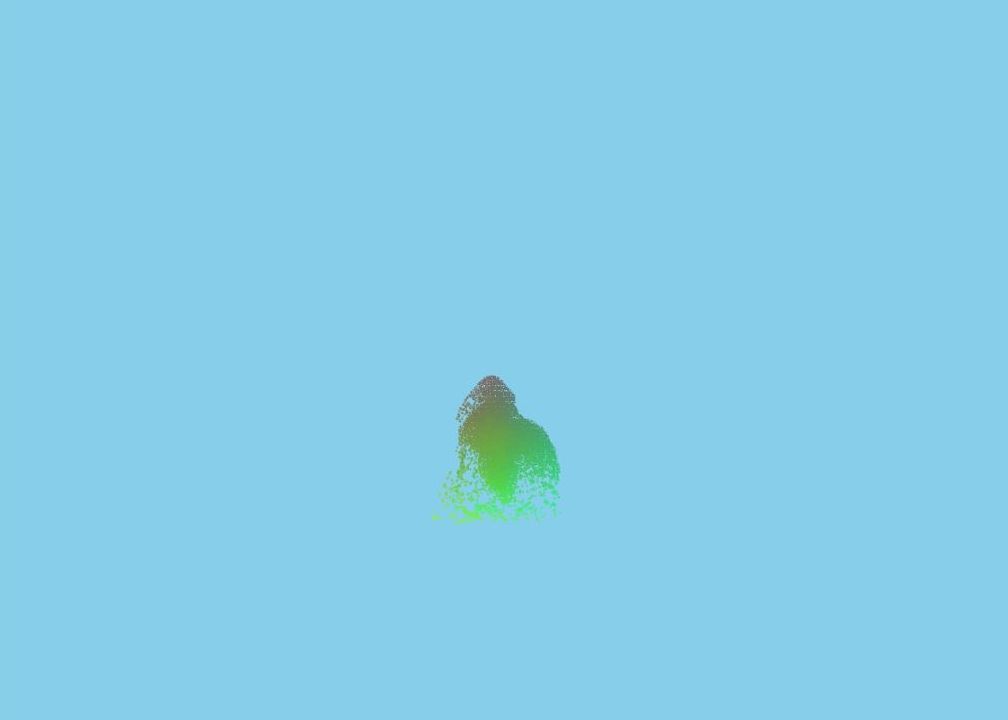
\includegraphics[width=1\columnwidth]{Bilder/1.jpg}
\end{figure}
\begin{figure}[H]
	\centering
	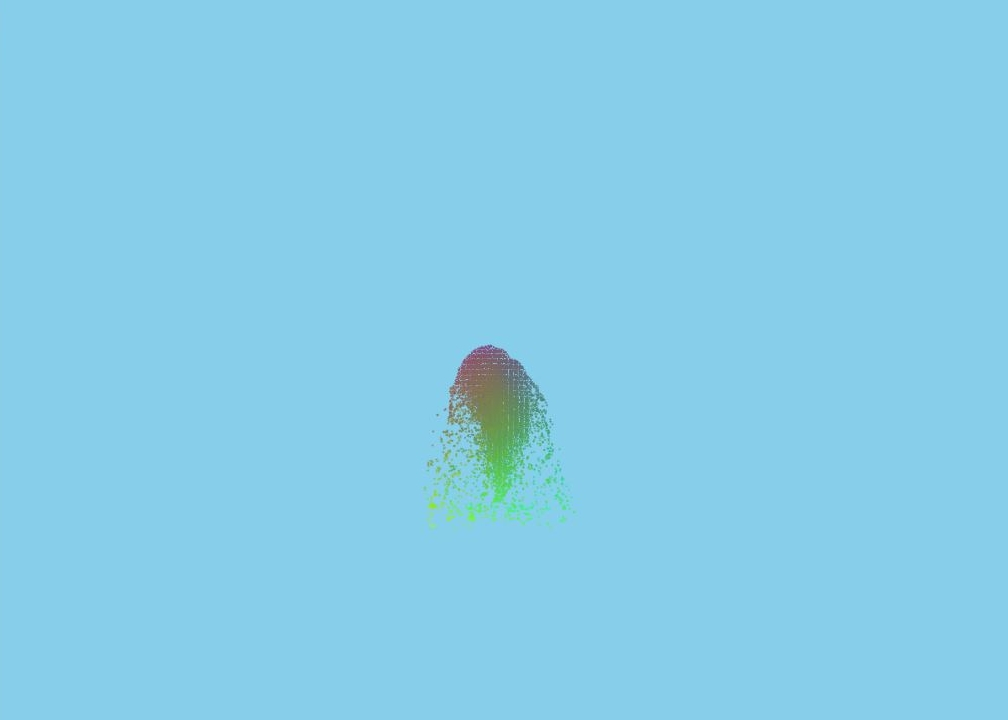
\includegraphics[width=1\columnwidth]{Bilder/2.jpg}
\end{figure}
\begin{figure}[H]
	\centering
	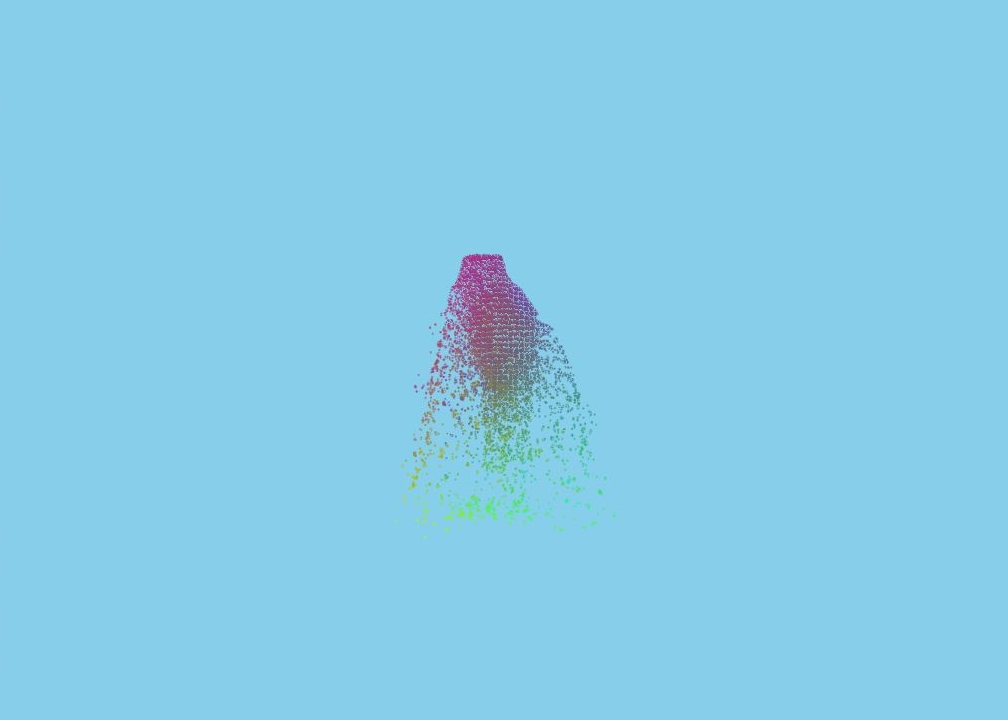
\includegraphics[width=1\columnwidth]{Bilder/3.jpg}
\end{figure}
\begin{figure}[H]
	\centering
	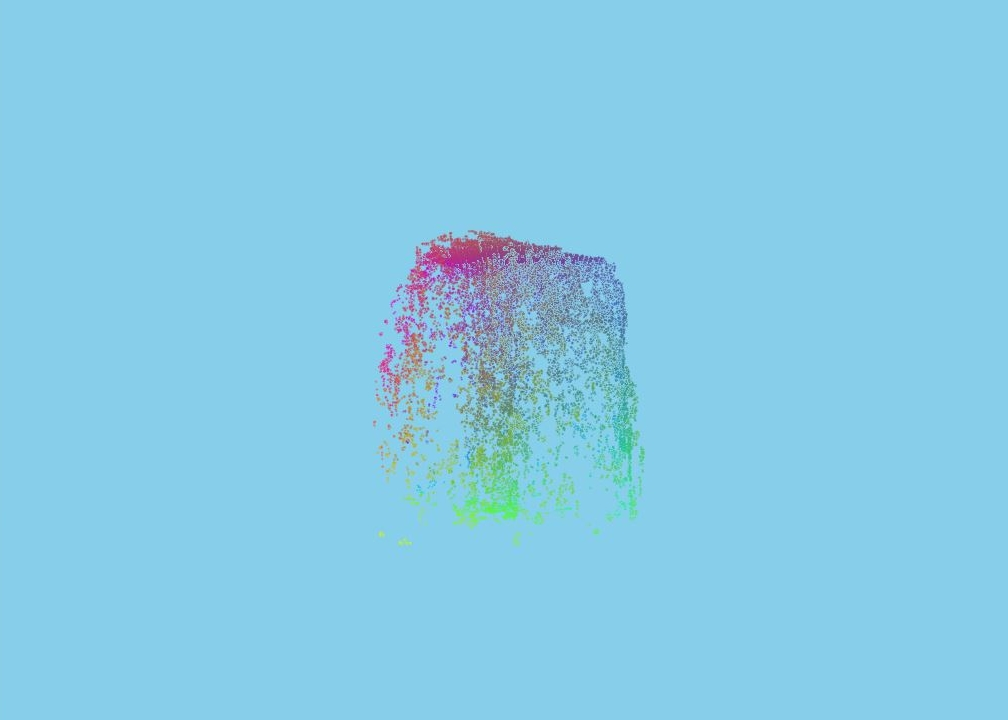
\includegraphics[width=1\columnwidth]{Bilder/4.jpg}
\end{figure}
\begin{figure}[H]
	\centering
	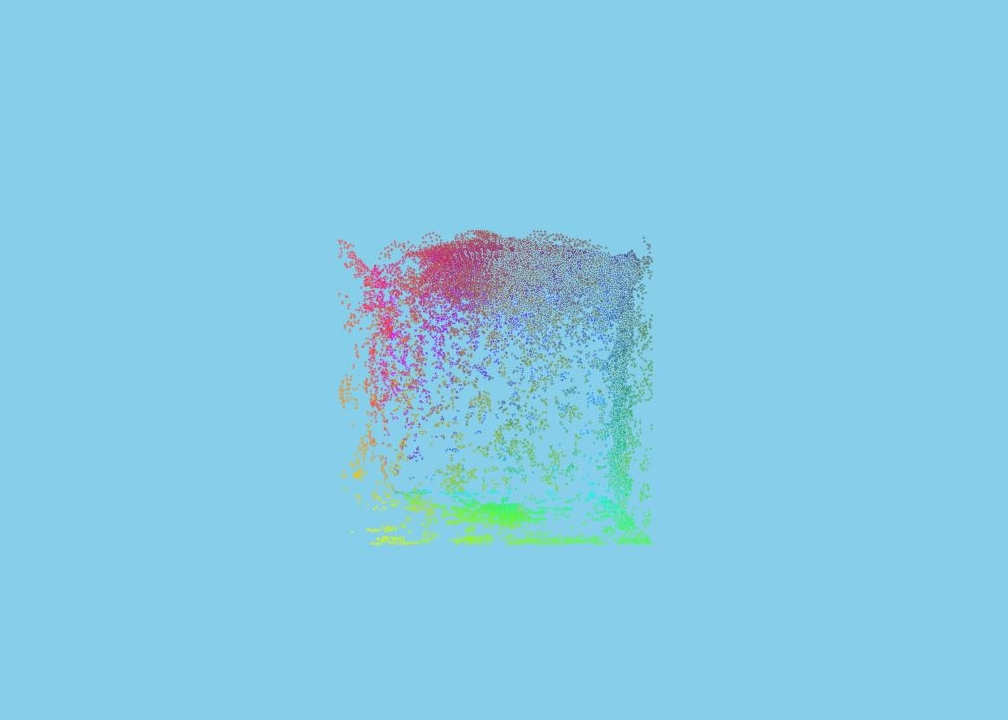
\includegraphics[width=1\columnwidth]{Bilder/5.jpg}
\end{figure}
\begin{figure}[H]
	\centering
	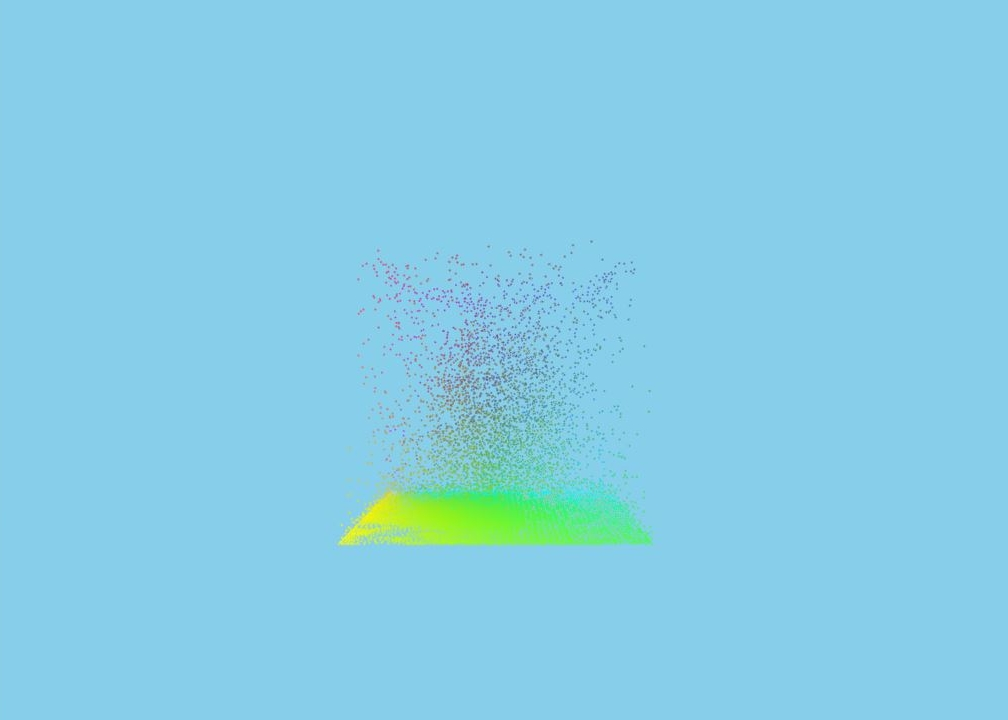
\includegraphics[width=1\columnwidth]{Bilder/6.jpg}
	\caption{Simulationsverlauf des Rauches}
\end{figure}

\section{Ausblick}\label{img:ausblick}

Die vorliegende Fluidsimulation bietet viele Möglichkeiten zur Erweiterung. Eine davon wäre die Realisierung einer Technik zur besseren Berechnung der Wirbelkraft, da diese einen großen optischen Einfluss auf die Simulation hat. Diese könnte durch das Einbringen von Vektorfeldern oder einer ähnlichen Technik erfolgen. Vorteilhaft wäre es, wenn diese als Coroutine, unabhängig von der der Berechnung der Partikelinteraktionen, berechnet werden könnte. Dadurch müsste diese nicht bei jedem Frame, sondern könnte in einem festen Intervall berechnet werden, um entsprechend Leistung zu sparen.
\newline
Außerdem wurden bisher nur Point-Sprites gerendert, welche kein aufwendiges Rendering benötigen, aber nicht besonders optisch ansprechend sind. Deshalb würde sich hier ein realistisches Rendern der Partikel anbieten. Dabei könnten die Point-Sprites durch Texturen ersetzt werden, wie es bei Partikelsimulationen in Unity üblich ist. Eine übliche Art des Renderings bei Fluiden wäre ein \textit{marching-cubes}-Algorithmus, welcher ein Mesh erstellen würde. Dies bedarf aber einen hohen Aufwand beim Erstellen des Meshes. Müller \cite{muller2007screen} schlägt aber alternativ ein \textit{screen-space-fluid}-Rendering, vor welches nur die nächstgelegen Oberfläche zur Kamera rendern würde. Dabei könnte gegenüber dem \textit{marching-cubes}-Algorithmus wichtige Laufzeit gespart werden.
\newline
Um weitere Verbesserungen in der Performance zu erreichen sollten noch andere Beschleunigungsverfahren in Betracht gezogen und gegeneinander abwägt werden. Außerdem sollten, weitere Anpassungen beim Countingsort in Zukunft sich auf dessen Beschleunigung auswirken. Da dieser, in Relation zur Partikelanzahl, keine lineare Laufzeit hat. Die genaue Ursache für diese Abweichung könnte untersucht und behoben werden.

\newpage
\listoffigures
\newpage
\bibliography{lib}

\end{document}